\section{Equazioni di Hamilton}

\begin{frame}{Hamiltoniana problema 2 corpi ridotto}

\begin{columns}

\begin{column}{0.2\textwidth}

\begin{figure}[!ht]

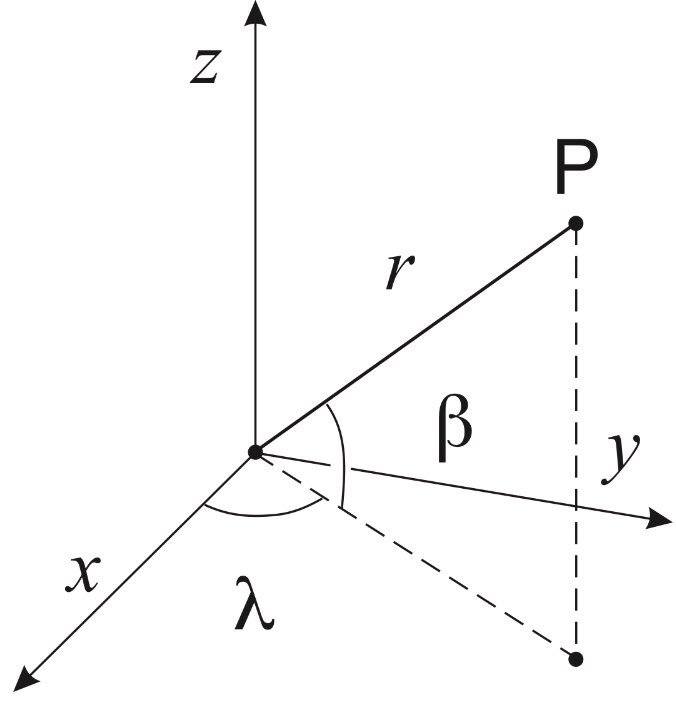
\includegraphics[width=\textwidth]{analytic}

\end{figure}


\end{column}

\begin{column}{0.8\textwidth}

\begin{align*}
&T=\frac{1}{2}\mu(\dot{r}^2+r^2\dot{\beta}^2+r^2\cos{\beta}^2\dot{\lambda}^2)\\
&V=-k^2\frac{\mu}{r}\\
&L=T-V
\end{align*}

\end{column}

\end{columns}

\begin{block}{Momenti coniugati}

\begin{align*}
&p_r=\PDy{\dot{r}}{L}=\mu\dot{r}\\
&p_{\beta}=\PDy{\dot{\beta}}{L}=\mu r^2\dot{\beta}\\
&p_{\lambda}=\PDy{\dot{\lambda}}{L}=\mu r^2\cos{\beta}^2\dot{\lambda}\quad \dot{p}_{\lambda}=0
\end{align*}

\end{block}

\begin{block}{Hamiltoniana}

\begin{align*}
&H(p,q)=\frac{1}{2\mu}(p_r^2+\frac{1}{r^2}p_{\beta}^2+\frac{1}{r^2\cos{\beta}^2}p_{\lambda}^2)-\frac{k^2\mu}{r}
\end{align*}


\end{block}

\end{frame}

\begin{wordonframe}{Meccanica Hamiltoniana}

\begin{block}{Equazioni di Hamilton}
\begin{align*}
&\dot{q}=\PDy{p}{H}\\
&\dot{p}=-\PDy{q}{H}
\end{align*}
\end{block}

$\TDy{t}{H}=\PDy{t}{H}$

\end{wordonframe}


\section{Equazione di Hamilton-Jacobi}

\begin{block}{Trasformazioni canoniche}

\begin{align*}
(p,q)\to(\xi(p,q),\eta(p,q))
\end{align*}

che lasciano invariate le equazioni di Hamilton.

\end{block}

\begin{block}{Problema di H-J}

Trovare trasformazione canonica tale che $K=0$: $(\xi,\eta)$ sono costanti del moto.

\end{block}

\begin{block}{Funzione generatrice $S(q,\eta,t)$}

\begin{align*}
&\xi=\PDof{\eta}S(q,\eta,t)\ (2: \xi(p,q))\\
&p=\PDof{q}S(q,\eta,t)\ (1:\eta(q,p))\\
&K=H+\PDy{t}{S}\ K=0\Leftrightarrow H(q,\PDy{q}{S},t)=-\PDy{t}{S}
\end{align*}


\end{block}

\begin{frame}{Soluzione dell'equazione di H-J}

\begin{align*}
\frac{1}{2\mu}[(\PDy{r}{S})^2+\frac{1}{r^2}(\PDy{\beta}{S})^2+\frac{1}{r^2\cos^2{\beta}}(\PDy{\lambda}{S})^]-\frac{k^2\mu}{r}=-\PDy{t}{S}
\end{align*}

Un integrale completo contiene tante variabili quanti sono i gradi di libert\'a: le $\eta$.

\begin{block}{L'equazione di H-J \'e separabile}

\begin{align*}
S(r,\beta,\lambda,t)=S_r(r)+S_{\beta}(\beta)+S_{\lambda}(\lambda)-\sigma t\\
\end{align*}

\begin{columns}

\begin{column}{0.5\textwidth}

Variabili canoniche $J_{\phi}, J_{\chi}, J_{\psi}$

\begin{align*}
&\PDy{J_{\phi}}{S}=\phi-nt\\
&\PDy{J_{\chi}}{S}=w-v=\chi\\
&\PDy{J_{\psi}}{S}=\lambda-\bar{\lambda}=\psi
\end{align*}


\end{column}

\begin{column}{0.5\textwidth}

Variabili canoniche $E, J, J_{\lambda}$

\begin{align*}
&S_{\lambda}=J_{\lambda}\lambda\\
&S_{\beta}=Jw-J_{\lambda}\bar{\lambda}\\
&S_r=ku\sqrt{a}(u+e\sin{u})-ku\sqrt{p}v\\
&\PDy{E}{S_r}=\frac{\phi}{n} \ \PDy{J}{S_r}=-v
\end{align*}

\end{column}

\end{columns}



\end{block}


\end{frame}


\section{Sistemi integrabili e degenerazione}

\begin{frame}{Teorema di Liuville-Arnol'd}

Se in un sistema Hamiltoniano con n gradi di libert\'a sono noti n integrali primi del moto indipendenti ed in involuzione (parentesi di Poisson nulle) allora esiste una trasformazione canonica nelle variabili angolo-azione nella quale H dipende solo dalle variabili azione mentre le variabili angolo evolvono linearmente nel tempo. Le equazioni del moto potranno essere risolte tramite quadratura.


\end{frame}

\begin{wordonframe}{Integrabilit\'a EOM}

\begin{align*}
\frac{dq_1}{\sqrt{2(hf_1-v_1+c_1)}}=\ldots=\frac{dq_n}{\sqrt{2(hf_n-v_n+c_n)}}=\frac{dt}{f}=d\tau
\end{align*}

\end{wordonframe}

\begin{frame}{Periodi del moto}

Quando i periodi indipendenti sono meno dei gradi di libert\'a si parla di degenerazione: \'e connessa con la possibilit\'a di scegliere in pi\'u modi le 3 costanti del moto del teorema di L-A.

\end{frame}
